\chapter{Grundlegendes Konzept}

\section{Aufbau einer Webanwendung}
\label{cha:webapplication_structure}

Das Konzept der Schichtenarchitektur ist in der Softwareentwicklung eine Client-Server-Architektur, welche die Darstellung, Anwendungslogik und Datenverwaltung physikalisch trennt.  
Das Konzept der abgestuften Architektur bei der Anwendungsentwicklung lässt sich von einem 1-Stufen-Ansatz bis hin zu einem n-Stufen-Ansatz einteilen. Jeder dieser Ansätze hat seine Vorzüge, doch für eine webbasierte Anwendung eignet sich der n-Stufen-Ansatz. Das Grundkonzept einer solchen Architektur besteht darin, eine Anwendung in unabhängige Ebenen mit definierten Rollen aufzuteilen.
Die mehrstufige Anwendungsarchitektur ermöglicht es den EntwicklerInnen flexible, wiederverwendbare und austauschbare  Anwendungskomponenten zu erstellen, welche zu einer Schichtenanwendung verknüpft werden können, ohne die komplette Endanwendung umschreiben zu müssen.
Diese mögen sich auf der selben Maschine befinden, werden aber meist auf unterschiedliche ausgelagert \cite{wiki-ntier-architecture}.

Beispielsweise sind bei dem 1-Stufen-Ansatz alle für die Anwendung relevanten Funktionen -- Darstellung, Logik, Datenverwaltung, \etc -- auf der Client-Maschine vereint. Durch die Limitierung, dass die komplette Software auf einem Gerät betrieben wird und die daraus folgenden Skalierungsprobleme, ist dieser Ansatz kaum für Webanwendungen geeignet.
Der gebräuchlichste Stufenansatz ist der 3-stufige, siehe Abb.~\ref{fig:3-stufen-architektur}, welcher in der Regel Darstellung, Anwendungslogik und Datenverwaltung entkoppelt. Ein Webbrowser, zur Anzeige der Benutzeroberfläche, wäre zum Beispiel die erste Stufe. Ein Webserver, welcher die Logik ausführt, die Zweite und als dritte Ebene, zur Datenverwaltung, käme eine Datenbank in Frage. 

Obwohl der 3-Stufen-Ansatz die Skalierbarkeit erhöht und eine Trennung der Anwendungslogik von den Anzeige- und Datenverwaltungsschichten einführt, trennt er die Anwendung nicht wirklich in spezialisierte Schichten. Für Prototyp- oder einfache Webanwendungen kann eine dreistufige Architektur ausreichen. Bei komplexen Anforderungen an solche Anwendungen ist ein 3-stufiger Ansatz jedoch in mehreren Schlüsselbereichen, einschließlich Flexibilität und Skalierbarkeit, unzureichend, und es wäre sinnvoll, einen n-Stufen-Ansatz zu wählen \cite{nTier-architecture}.

Der größte Nachteil von diesen Ansätzen ist der zusätzliche Overhead-Aufwand  und eine höhere Latenz, was wiederum die der NutzerInnen wahrgenommen Geschwindigkeit mindert.

Die Trennung von Logik ist in der Webentwicklung ein wesentliches Konzept. Wie in diesem Kapitel die Abstraktion durch Stufen, oder Ebenen, wird im folgenden Kapitel \ref{cha:component_usage} die Trennung von Logik, mittels Komponenten, behandelt.

\begin{figure}
	\centering
	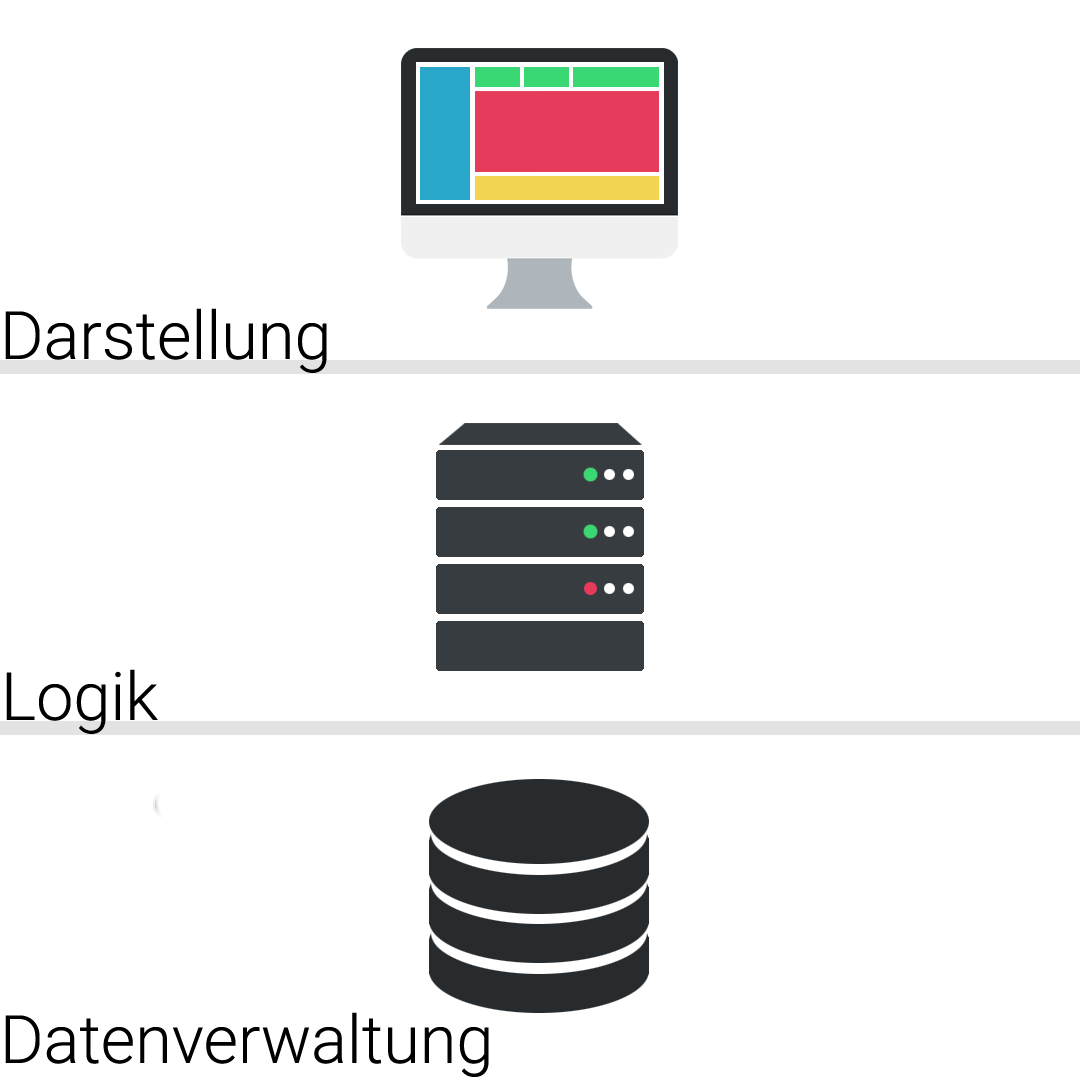
\includegraphics[width=0.5\linewidth]{images/3-stufen-architektur}
	\caption{3-Stufen-Architektur}
	\label{fig:3-stufen-architektur}
\end{figure}

\section{Verwendung von Komponenten im Web}
\label{cha:component_usage}
%TODO How to gender EntwicklerIn, der/des entwicklers?
%TODO Darf man das Beispiel 1:1 reproduzieren ?
Das Web besteht aus Bausteinen, sogenannten Elementen. Wenn EntwicklerInnen beispielsweise einen Link mittels einem a-Tag nutzen, wird erwartet, dass dieser sich wie ein Link-Element verhält. Dieses Element hat seine eigene standardmäßige blaue Farbe, einen Handzeiger bei hover und vor allem die Funktionalität, dass bei einem Klick auf das Element zu einer neuen URL weitergeleitet wird. Dieses Verhalten und Styling wird ohne jegliches einwirken des/der EntwicklerIn bereitgestellt. Jedes HTML Element funktioniert nach diesem Prinzip, welches HTML Code einfacher zu schreiben, aber auch verständlicher macht.
Durch Kombination solcher Elemente, mit eigens definierten Stylesheets können komplexere Gerüste aus HTML Elementen, mit komplexeren CSS/Javascript entstehen.

Damit nicht ein/eine EntwicklerIn die komplette Struktur im Kopf behalten muss, und bei Problemen nur diese/r das aufgetretene Problem beheben kann, hat sich bewehrt, Code in kleine, überschaubare Teile herunter zu brechen, in Einheiten, welche das gesamte Gerüst wartbar machen. Diese Teile können einfachere Funktionen, Module, Komponenten oder aber viele andere Ansätze sein, welche komplexe Strukturen in atomare Einzelteile aufteilen \cite{components-benefit}.

Um also die Definition der, in dieser Arbeit fokussierten Technologie -- einer Komponente -- zusammen zu fassen: Eine entkoppelte Sammlung von Funktionalität oder Prozessen und Logik, mit einer verständlichen Schnittstelle oder API um des Komponenten Funktionalität abzurufen.

\section{Anforderung an die komponentenorientierte Webanwendung}

\section{Eigene Idee, technisches Design}
